\documentclass[handout,10pt]{beamer}

\usepackage{beamerthemesplit}
\usepackage{pgfpages}
\usepackage{verbatim}
\usepackage{fancybox}

%\usepackage{algorithmic}
\usepackage{amsmath}
\usepackage{listings}
\usepackage{amsthm}
\usepackage{algorithm2e}
\usepackage{algorithmic}
\usepackage{lipsum}% http://ctan.org/pkg/lipsum
\usepackage{xifthen}% http://ctan.org/pkg/xifthen
\usepackage{needspace}% http://ctan.org/pkg/needspace
\usepackage{hyperref}% http://ctan.org/pkg/hyperref

\newcommand\Small{\fontsize{9}{9.2}\selectfont}
\newcommand*\LSTfont{\Small\ttfamily\SetTracking{encoding=*}{-60}\lsstyle}

\lstset{language=C,
numberstyle=\footnotesize,
basicstyle=\tiny\ttfamily,
stepnumber=1,
fontstyle=\small,
frame=shadowbox,
breaklines=true}

\newcommand{\field}[1]{\mathbb{#1}} %requires amsfonts

% Multiple pages...
%\pgfpagesuselayout{4 on 1}

\usetheme{Antibes}
\usecolortheme{beaver}
\title[Team Satisfaction - $3$-$SAT$]{The $3$-$SAT$ Decision Problem \\ Towards a Parallel Search Implementation}

\usepackage{mathptmx}
\usepackage[scaled=.90]{helvet}
\usepackage{courier}
\usepackage[T1]{fontenc}

%\pgfpagesuselayout{4 on 1}[letterpaper,border shrink=5mm]

\institute[RIT]{}
\date{\today}
\subtitle{Team Satisfaction}
\author{Christopher Wood, Eitan Romanoff, Ankur Bajoria}
%\institute[]{}
\date{\today}

\begin{document}

\begin{frame}
	\titlepage
\end{frame}

\begin{frame}
	\frametitle{Agenda}
	\tableofcontents
\end{frame}

\section{Problem Statement}
\begin{frame}
	\frametitle{Boolean Satisfiability}

	Boolean satisfiability is an $NP$-complete decision problem defined as:
	\begin{align*}
	SAT : \phi \to \{YES, NO\}
	\end{align*}

	\medskip

	\textbf{Input}: Boolean formula $\phi_n$ on $n$ variables.
	
	\begin{align*}
		\phi_5 = (x_1 \lor x_2 \lor \lnot x_3) \lor \lnot x_4 \land x_5 \land (\lnot x_2 \lor x_3 \land (x_4 \land x_1))
	\end{align*}

	\medskip 

	\textbf{Output}: $YES$ if there exists a truth assignment to the
	variables in $\phi_n$ such that it evaluates to true, $NO$ otherwise.

	\medskip

	\begin{center}
		$\phi_n$ is satisfiable $\Leftrightarrow$ $SAT(\phi_n) = YES$
	\end{center}

\end{frame}

% TODO: give a sample circuit of the problem

\begin{frame}
	\frametitle{$3$-$SAT \in NP$}
	\begin{itemize}
		\item A special case of $SAT$ that fixes the format of $\phi_n$.
		\item Each input formula is in $3$-$CNF$ form:
		\begin{itemize}
			\item The conjunction (Boolean AND) of arbitrarily many clauses, 
			where each clause is the disjunction (Boolean OR) of exactly three literals 
			(a Boolean variable or its negation).
			\begin{align*}
				(x_1 \lor x_2 \lor \lnot x_3) \land (\lnot x_1 \lor x_2 \lor x_3) \land (\lnot x_1 \lor x_2 \lor \lnot x_3)
			\end{align*}
		\end{itemize}
		\item $SAT$ reduces to $3$-$SAT$, so $3$-$SAT \in NP$.
	\end{itemize}
\end{frame}

% TODO: give example of 3-CNF formula
% Introduce the team members.
% Briefly describe your NP problem.
% Briefly describe the exhaustive search algorithm for your problem.

\section{Exhaustive Search Algorithm}
\begin{frame}[fragile]
	\frametitle{Exhaustive Search for $3$-$SAT$}
\textbf{Input:} $3$-$CNF$ formula $\phi_n$ on $n$ variables, \textbf{Output:} YES or NO 

\medskip

\begin{algorithm}[H]
\begin{algorithmic}[1]
\STATE $C \gets FALSE^n$ (array of $n$ False values, the initial configuration)
\FOR{$i = 0 \to 2^n - 1$}
	\STATE $SAT \gets TRUE$
	\FORALL{$clause \in \phi_n$}
		\IF{$evaluate(clause, C) = FALSE$}
			\STATE $SAT \gets FALSE$
		\ENDIF
	\ENDFOR	
	\STATE \textbf{if} $SAT = TRUE$ \textbf{then return} $YES$
	\STATE $C \gets nextConfig(C)$
\ENDFOR
\RETURN $NO$
\end{algorithmic}
%\caption{Exhaustive search for $3$-$SAT$.}
\label{alg:seq}
\end{algorithm}
	
%	input: 
%	for each $2^n$ variable configuration
%		assign variable to literals in $\phi$ 
%		evaluate $\phi$
%		if (true) return YES
%	return NO
\end{frame}

\begin{frame}
	\frametitle{Exhaustive Search for $3$-$SAT$ - A \emph{Very Satisfiable} Example!}
\textbf{Input}: $\phi_5 = (\lnot X_1 \lor \lnot X_2 \lor \lnot X_3) \land (X_3 \lor \lnot X_4 \lor \lnot X_5)$ \\
\textbf{Output}: Yes \\ 
\textbf{Note}: no early termination once a satisfiable solution is found
\begin{figure}
\centering
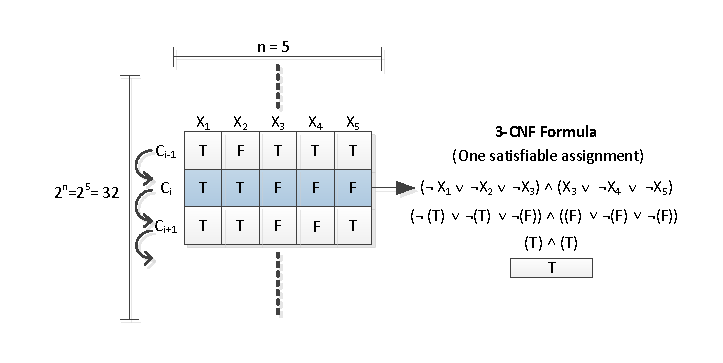
\includegraphics[scale = 0.8]{satSolverAlg.pdf}
\end{figure}
	% image of how the algorithm works 
	% Array of truth values on left, arrows that point to literals, and then output truth value on the right
\end{frame}

\begin{frame}[fragile]
	\frametitle{Evaluating a Clause}
\begin{itemize}
	\item Evaluating a clause depends on how $\phi_n$ and the variable truth assignments are stored.
	\begin{itemize}
		\item {\tt boolean[] variables} for variable assignments and {\tt Literal[][3] formula} for $\phi_n$.
		\item A {\tt Literal} has a variable ID and negated flag
	\end{itemize}
\end{itemize}
{\small
\begin{lstlisting}
for (int c = 0; c < numClauses; c++) {
    boolean clauseValue = false;
    for (int l = 0; l < 3 && clauseValue == false; l++) {
        if (formula[c][l].negated == true && !variables[formula[c][l].id])
            clauseValue = true;
        else if (formula[c][l].negated == false && variables[formula[c][l].id])
            clauseValue = true; 
    }
    // Check the value of the clause now...
}
\end{lstlisting}
}
\end{frame}

\section{Advanced Techniques and Heuristics for Parallel SAT Algorithms}
% Describe the algorithm from your first research paper.
\begin{frame}
	\frametitle{Recursive Divide and Conquer with CUDA}
	\begin{itemize}
		\item Idea: Recursively search the variable assignment space
		\item Approach: A formulas is a ``stack'' of clauses that are reduced or popped off during assignment 
		\item Implementation: Master-worker pattern for distributing formulas to individual CUDA kernels
	\end{itemize}
\begin{figure}
\centering
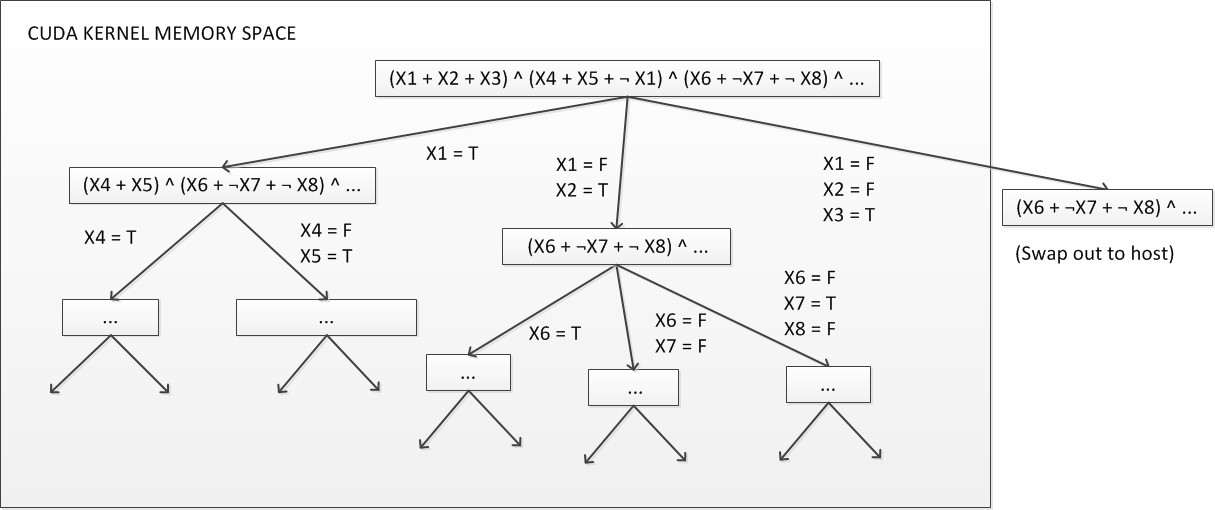
\includegraphics[scale = 0.30]{satDCswap.jpg}
\end{figure}
\end{frame}

% Describe the algorithm from your second research paper.
\begin{frame}
	\frametitle{Advanced Clause Learning and Sharing with ManySAT}
	\begin{itemize}
		\item Idea: Exploit heuristics for particular types of formulas
		\item Approach: Run multiple sequential solvers in parallel and reduce the result together
		\item Implementation: Each solver uses different restart policies, literal selection strategies, and shared
		conflict-driven clause learning 
	\end{itemize}
\begin{figure}
\centering
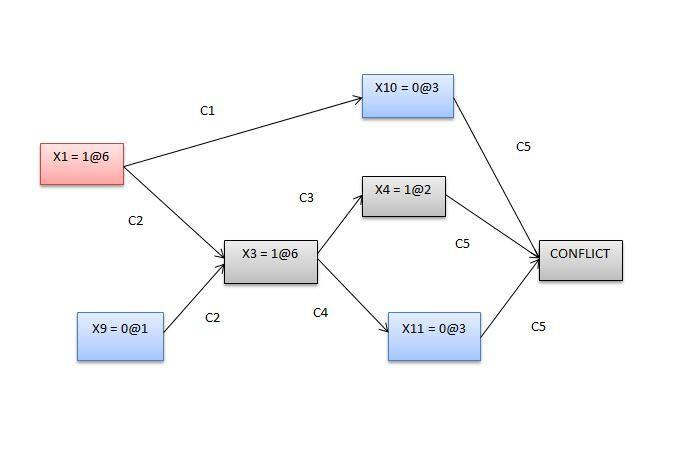
\includegraphics[scale = 0.32]{implication.jpg}
\end{figure}
\end{frame}

% Describe the algorithm from your third research paper.
\begin{frame}
	\frametitle{Intelligent Literal Decisions and Advanced Data Structures for DPLL}
	\begin{itemize}
		\item Idea: Enhance literal selection to more effectively traverse the search space
		\item Approach: Use trie data structures to build ``guided paths'' that indicate whether a branch has been visited or not
		\item Implementation: Distribute guided paths across different worker processes using a master-worker pattern
	\end{itemize}
\begin{figure}
\centering
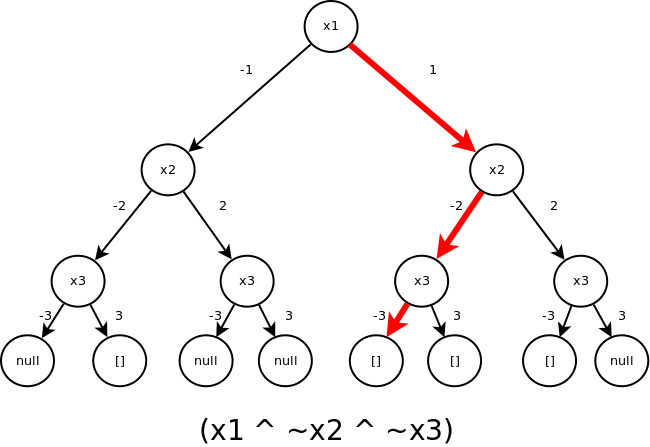
\includegraphics[scale = 0.2]{trie.png}
\end{figure}
\end{frame}

\section{Parallel Program Design and Demonstration}
% Describe the design of your parallel program.
\begin{frame}
	\frametitle{Parallel Program Characteristics}
	Our design goals included:
	\begin{itemize}
		\item Evenly divide the computation among different threads
		\item Minimize (or remove) conlficts for shared variables
	\end{itemize}

	\medskip

	Our parallel design strategy:
	\begin{itemize}
		\item \emph{Result parallelism} for exhaustive program and \emph{agenda parallelism} for decision program
		\item Split the evaluation of each variable configuration among every thread
		\item Reduce the final result into the main thread
		\item Balance the load using a guided schedule
	\end{itemize}
\end{frame}

% TODO: include a slide about the variables and how we split them?
% \begin{frame}
% 	\frametitle{The Parallel Transformation}
% 	Managing variable access
% \begin{table}
% 	\begin{tabular}{c | c | c}
% 	Sequential Variable & Parallel Variable & Shared? \\ \hline
% 	Literal[][] & ~ & ~ \\
% 	configuration[] & ~ & ~ \\
% 	numSatisfiable & ~ & ~ \\
% 	~ & ~ & ~ \\
% 	~ & ~ & ~ \\
% 	\end{tabular}
% \end{table}
% \end{frame}

\begin{frame}
	\frametitle{Computation Partition Strategy}
\begin{figure}
\centering
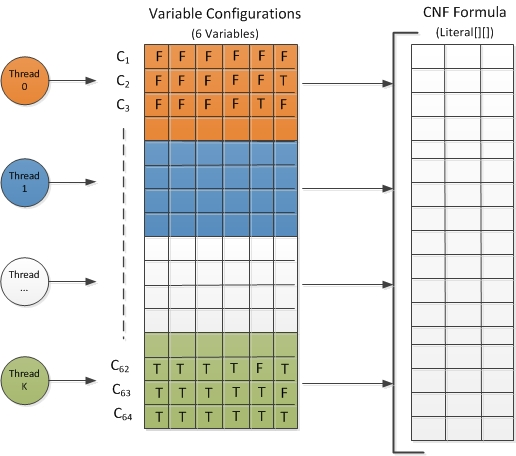
\includegraphics[scale = 0.5]{teamdesign.jpg}
\end{figure}
\end{frame}

\begin{frame}
	\frametitle{Thread Synchronization}
\vspace{-1em}
\begin{figure}
\centering
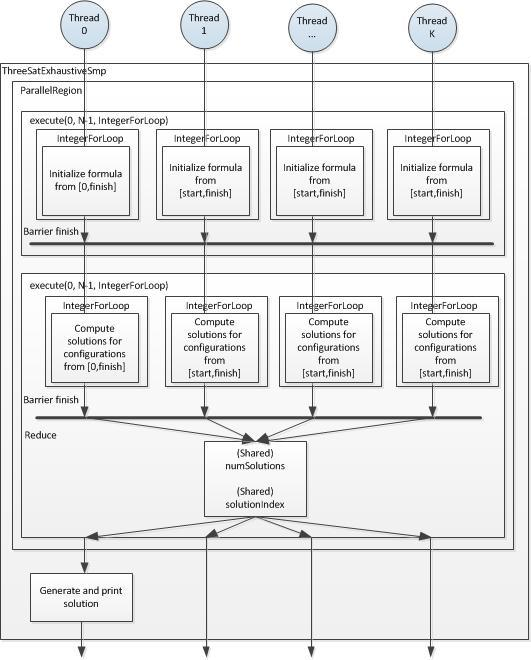
\includegraphics[scale = 0.29]{design.jpg}
\end{figure}
\end{frame}

% Give a brief demo of your parallel program for your problem, on a small instance of your problem.
\begin{frame}
	\frametitle{Action!}
	\begin{center}
		Demo time!
		\begin{align*}
			\phi_5 = (\lnot X_1 \lor \lnot X_2 \lor \lnot X_3) \land (X_3 \lor \lnot X_4 \lor \lnot X_5)
		\end{align*}
	\end{center}
\end{frame}

\section{Exhaustive Performance Metrics}
% Describe the performance metrics you measured.
\begin{frame}
	\frametitle{Speedup Metrics (Exhaustive)}

\begin{columns}
\column{.5\textwidth}
	\vspace{-1em}
	\begin{figure}
	\centering
	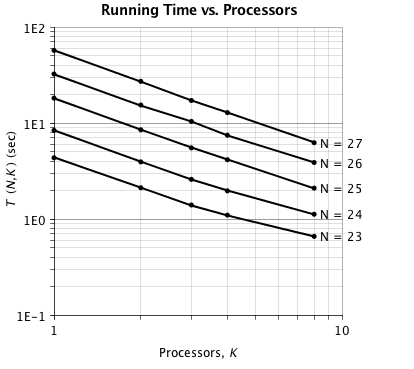
\includegraphics[scale = 0.25]{ge_speed_4.png}
	\end{figure}
	\vspace{-2em}
	\begin{figure}
	\centering
	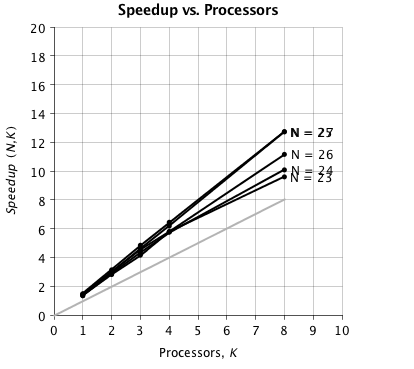
\includegraphics[scale = 0.25]{ge_speed_3.png}
	\end{figure}
\column{.5\textwidth}
\begin{minipage}[c][.6\textheight][c]{\linewidth}
	\vspace{-1em}
	\begin{figure}
	\centering
	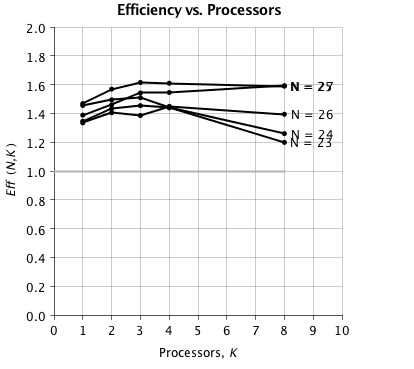
\includegraphics[scale = 0.25]{ge_speed_2.png}
	\end{figure}
	\vspace{-2em}
	\begin{figure}
	\centering
	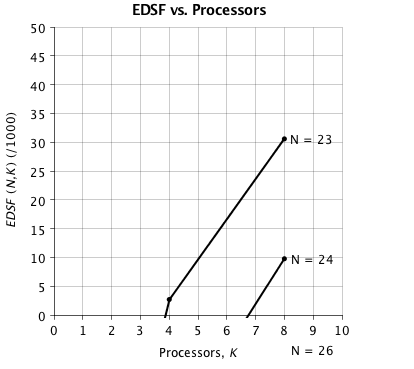
\includegraphics[scale = 0.25]{ge_speed_1.png}
	\end{figure}
\end{minipage}
\end{columns}
\end{frame}

\begin{frame}
	\frametitle{Sizeup Metrics (Exhaustive)}
\begin{columns}
\column{.5\textwidth}
	\vspace{-1em}
	\begin{figure}
	\centering
	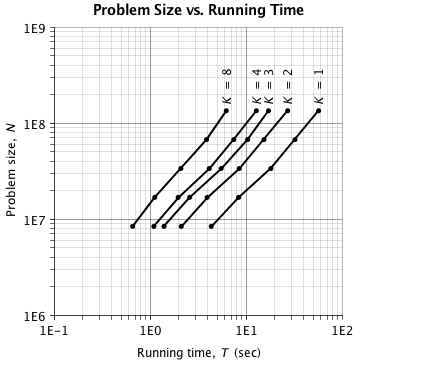
\includegraphics[scale = 0.25]{ge_size_4.png}
	\end{figure}
	\vspace{-2em}
	\begin{figure}
	\centering
	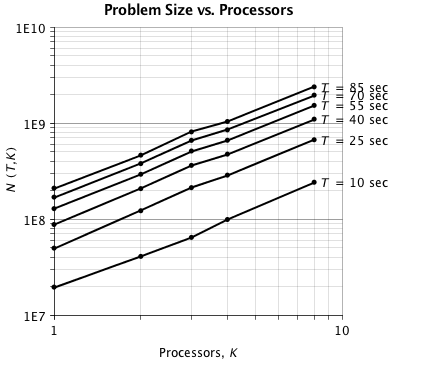
\includegraphics[scale = 0.25]{ge_size_3.png}
	\end{figure}
\column{.5\textwidth}
\begin{minipage}[c][.6\textheight][c]{\linewidth}
	\vspace{-1em}
	\begin{figure}
	\centering
	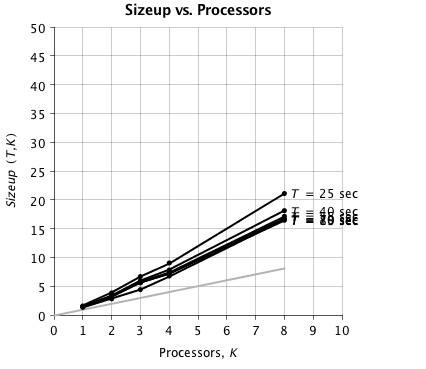
\includegraphics[scale = 0.25]{ge_size_2.png}
	\end{figure}
	\vspace{-2em}
	\begin{figure}
	\centering
	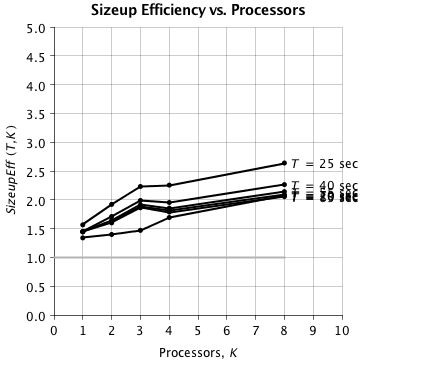
\includegraphics[scale = 0.25]{ge_size_1.png}
	\end{figure}
\end{minipage}
\end{columns}
\end{frame}

\begin{frame}
	\frametitle{Performance Observations}
	\begin{itemize}
		\item We achieved \emph{superlinear} speedups and sizeups using a guided schdule with varying the number of variables
		\item Exaustive 3-SAT problems have implicit unbalanced loads
		\begin{itemize}
			\item A guided schedule yielded the best results for speedup and sizeup
			\item A dynamic schedule caused a \emph{significant} amount of overhead
		\end{itemize}
		\item Our parallel programs achieve better performance when the number of variables was varied:
		\begin{itemize}
			\item The problem size $N = f(N_v, N_c) = 2^{N_v} \times N_c$
		\end{itemize}
	\end{itemize}
\end{frame}

\section{Lessons Learned and Future Work}
% Discuss what you learned from your investigation.
% Discuss future work that could be done to further your investigation.
\begin{frame}
	\frametitle{Lessons Learned}
	\begin{itemize}
		\item If the problem size is a function of \emph{multiple} variables, experiments should only change one 
		of such variables to gather valid performance data
		\item A guided schedule yielded the most balanced load for our computation partition strategy
		\item Exploiting the cache and JVM can yield \emph{extremely} good speedup and sizeup efficiencies
	\end{itemize}
\end{frame}

\begin{frame}
	\frametitle{Future Work}
	\begin{itemize}
		\item Implement more advanced heuristics for literal selection
		\item Strive for wider splits of the configuration search space tree among multiple processes 
		\item Experiment with different data structures to see what's the most optimal
	\end{itemize}
\end{frame}

\section{Questions}
\begin{frame}
	\frametitle{Questions?}
	\begin{center}
		Fire away!
	\end{center}
\end{frame}

\begin{comment}
\begin{figure}
\centering
\includegraphics[scale = 0.6]{images/sub_layer.jpg}
\end{figure}
\end{comment}

\end{document}
